
\chapter{Metodología seguida en el desarrollo del trabajo} % Título del capítulo

\label{Metodología} % etiqueta \ref{Metodología}

\section{Descripción de tareas, fases y procedimientos}

Se procede a describir la metodología llevada a cabo para el desarrollo de este proyecto.
Se diferencian 4 fases incluyendo diferentes tareas en cada fase.
La primera y la cuarta fase son transversales a todo el proyecto.
Sin embargo, la ejecución de la tercera fase depende de la finalización de la segunda.
Además, tanto la segunda como la tercera fase dependen de los conocimientos establecidos en la primera.

\subsection{Fase 1. Recursos de desarrollo hardware y software}

\subsubsection{Descripción}

Esta fase tiene como objetivo afianzar los conocimientos relativos a las plataformas de desarrollo hardware y software que se han utilizado durante la elaboración del proyecto, así como consolidar el uso de herramientas de control de versiones y la metodología de integración continua para la gestión eficaz del código empleado.

\subsubsection{Recursos}

\label{recurs}

\begin{itemize}
\item \textbf{Recursos hardware}
    \begin{itemize}
        \item Dos PCs (Laboratorio y personal)
        \item FPGAs:
            \begin{itemize}
                \item Una Xilinx Artix-7 35T; Placa Digilent Arty A7 (Laboratorio)
                \item Dos Xilinx Artix-7 100T; Placa Digilent Arty A7 (Laboratorio y personal)
                \item Una Lattice ICE40 \footnote{Su uso ha sido minoritario. No obstante, se ha realizado algún test con ella, ver \href{https://github.com/stnolting/neorv32/issues/726}{\#726}}; Placa Alhambra II (Personal)
            \end{itemize}
        \item Servido Orion\footnote{Se ha empleado mayoritariamente para realizar implementaciones con Vivado.} (Laboratorio) 
    \end{itemize}
\item \textbf{Recursos software}
    \begin{itemize}
        \item FLOS:
            \begin{itemize}
                \item CuteCom
                \item GCC
                \item GHDL + GHDL yosys plugin
                \item Git + Gitk
                \item GTKWave
                \item Inkscape
                \item KolourPaint
                \item \LaTeX
                \item nextpnr-xilinx
                \item openFPGALoader
                \item Podman
                \item prjx-ray
                \item VUnit
                \item Wavedrom
                \item xed
                \item Yosys
            \end{itemize}
        \item Privativos:
            \begin{itemize}
                \item Vivado
            \end{itemize}
        \item Contenedores:
            \begin{itemize}
                \item docker.io/btdi/latex
                \item docker.io/ghdl/vunit
                \item docker.io/ghdl/vunit:mcode-master
                \item gcr.io/hdl-containers/impl/icestorm
                \item gcr.io/hdl-containers/sim/osvb
                \item ghcr.io/stnolting/neorv32/sim
                \item ghcr.io/unike267/containers/impl-arty
                \item ghcr.io/unike267/containers/latex-pygments
            \end{itemize}
        \item Plataformas
            \begin{itemize}
                \item GitHub
                \item GitLab
            \end{itemize}
        \item Lenguajes
            \begin{itemize}
                \item Bash
                \item C
                \item Markdown
                \item Python
                \item TCL
                \item TeX
                \item VHDL
                \item YML
            \end{itemize}
        \item Sistemas operativos:
            \begin{itemize}
                \item Fedora (Laboratorio)
                \item Linux Mint (Personal)
            \end{itemize}
    \end{itemize}
\end{itemize}

\subsubsection{Duración}

Transversal, de inicio a fin de proyecto, es decir, del 01/02/2024 al 30/09/2024.

\subsubsection{Tareas}

\noindent \textbf{\textit{Tarea 1}}

\textbf{Objetivo:} afianzar el uso de las herramientas software relativas al diseño hardware, su verificación y documentación. 

\textbf{Descripción:} con objeto de desarrollar el proyecto, se requieren los conocimientos necesarios para manejar con soltura las herramientas software referentes a la elaboración/simulación de VHDL tanto FLOS como privativas, a la síntesis/implementa- ción de VHDL tanto FLOS como privativas y a la compilación cruzada de programas de alto nivel, en concreto C, para ejecutar en RISC-V. 
Además, de ciertos conocimientos para desarrollar programas en python, así como para desarrollar documentos en markdown y \LaTeX.
En esta tarea, se adquieren estos conocimientos.


\noindent \textbf{\textit{Tarea 2}}

\textbf{Objetivo:} afianzar el uso de herramientas/metodologías para la gestión eficaz de código. 

\textbf{Descripción:} con objeto de gestionar de forma eficaz el código del proyecto, se requieren los conocimientos necesarios para utilizar la herramienta de control de versiones Git, complementada con las plataformas asociadas, así como dominar la metodología de integración continua en los repositorios en línea.
Para el caso de Git, se requiere manejar con soltura los comandos asociados para, entre otras cosas, generar/fusionar/eliminar ramas y hacer \textit{rebases} interactivos para reordenar/fusionar/eliminar \textit{commits}, además de realizar de forma correcta \textit{pull requests}.
Respecto a lo referente a la integración continua, se requieren los conocimientos relativos al desarrollo de archivos bash, como el realizado en \ref{ap-cod:23} para realizar la secuencia de comandos necesarios para la generación de \textit{bitstreams} mediante herramientas FLOS, así como los relativos al desarrollo de archivos TCL para realizar la secuencia de comandos necesarios para la generación de \textit{bitstreams} mediante Vivado, con objeto de incluir estos archivos a una lista de ejecución mediante código YML y así llevar a cabo la metodología de integración continua tanto en GitHub como en GitLab.
Asimismo, se ha de saber generar contenedores en CI, mediante un \textit{container file}, con objeto de realizar algunos de los contenedores necesarios para nuestras aplicaciones. 
En esta tarea, se obtienen estos conocimientos.

\subsection{Fase 2. Caracterización del rendimiento}

\subsubsection{Descripción}

En esta fase se han realizado todas las tareas referentes a la caracterización de los métodos de conexión con los que cuenta el NEORV32.
Ha sido la fase más prolongada y de ella ha dependido la fase 3.
A su vez, esta fase ha dependido del correcto aprendizaje de las herramientas necesarias adquirido a lo largo de la fase 1.

\subsubsection{Recursos}

Los mencionados en \ref{recurs}, excepto:

\begin{itemize}
    \item docker.io/btdi/latex
    \item ghcr.io/unike267/containers/latex-pygments
    \item Inkscape
    \item \LaTeX
\end{itemize}

\subsubsection{Duración}

Del 01/02/2024 al 12/06/2024.

\subsubsection{Tareas}

\noindent \textbf{\textit{Tarea 1}}

\textbf{Objetivo:} realizar el diseño de los multiplicadores a acoplar. 

\textbf{Descripción:} con objeto de tener un abanico de aceleradores a acoplar, se decide diseñar 3 multiplicadores con características diferentes.
En esta tarea, se realiza el diseño hardware y la simulación  de cada uno de estos coprocesadores.
Además, se realizan los \textit{wrappers} para AXI-Stream y Wishbone y se verifican con \textit{Verification Components}.
Las simulaciones se realizan mediante VUnit y se añaden a la integración continua del repositorio. 

\noindent \textbf{\textit{Tarea 2}}

\textbf{Objetivo:} realizar la conexión de los multiplicadores definidos mediante SLINK. 

\textbf{Descripción:} con objeto de testear el método de conexión Stream Link Interface (SLINK), se realiza la conexión de los tres multiplicadores mediante este método.
Para ello, se implementa en hardware el conjunto del diseño NEORV32 + Mult acoplado mediante SLINK y se verifica por UART.
La generación de los \textit{bitstreams} se realiza mediante Vivado, así como mediante herramientas FLOS y se añade a la integración continua del repositorio. 

\noindent \textbf{\textit{Tarea 3}}

\textbf{Objetivo:} realizar la conexión de los multiplicadores definidos mediante XBUS. 

\textbf{Descripción:} con objeto de testear el método de conexión Processor-External Bus Interface (XBUS), se realiza la conexión de los tres multiplicadores mediante este método.
Para ello, se implementa en hardware el conjunto del diseño NEORV32 + Mult acoplado mediante XBUS y se verifica por UART.
La generación de los \textit{bitstreams} se realiza mediante Vivado, así como mediante herramientas FLOS y se añade a la integración continua del repositorio. 

\noindent \textbf{\textit{Tarea 4}}

\textbf{Objetivo:} realizar la conexión de los multiplicadores definidos mediante CFS. 

\textbf{Descripción:} con objeto de testear el método de conexión Custom Functions Subsystem (CFS), se realiza la conexión de los tres multiplicadores mediante este método.
Para ello, se implementa en hardware el conjunto del diseño NEORV32 + Mult acoplado mediante CFS adaptando las fuentes del NEORV32 necesarias y se verifica por UART.
La generación de los \textit{bitstreams} se realiza mediante Vivado, así como mediante herramientas FLOS y se añade a la integración continua del repositorio. 

\noindent \textbf{\textit{Tarea 5}}

\textbf{Objetivo:} realizar la conexión de los multiplicadores definidos mediante CFU. 

\textbf{Descripción:} con objeto de testear el método de conexión Custom Functions Unit (CFU), se realiza la conexión de los tres multiplicadores mediante este método.
Para ello, se implementa en hardware el conjunto del diseño NEORV32 + Mult acoplado mediante CFU adaptando las fuentes del NEORV32 necesarias y se verifica por UART.
La generación de los \textit{bitstreams} se realiza mediante Vivado, así como mediante herramientas FLOS y se añade a la integración continua del repositorio. 

\noindent \textbf{\textit{Tarea 6}}

\textbf{Objetivo:} investigar sobre un método para realizar mediciones de latencia en el entorno NEORV32. 

\textbf{Descripción:} con objeto de hacer los ensayos de caracterización del rendimiento, se debe contar con un método generalizado para realizar las mediciones en simulación.
Se concluye que la medida mediante el CSR(mcycle) y la posterior extracción de su valor mediante \textit{external names} para plasmar su resultado a través de la función de VUnit \textit{info()}, es la opción más interesante.
En este sentido, también se planteó evaluar la señal \textit{valid} y \textit{ack} para los métodos AXI y Wishbone respectivamente, extrayendo en un CSV los \textit{time stamps} de los momentos en los que se daban estas señales y procesar estos valores mediante un programa en python.
No obstante, esta metodología era poco generalizable y se desechó la idea.
Sin embargo, para los ensayos del multiplicador aislado con \textit{Verification Components}, se ha utilizado este concepto.

\noindent \textbf{\textit{Tarea 7}}

\textbf{Objetivo:} realizar los ensayos de simulación para caracterizar el rendimiento de los métodos de conexión. 

\textbf{Descripción:} con objeto de caracterizar el rendimiento de los métodos de conexión, se plantean dos ensayos: de latencia y si es posible de \textit{throughput}.
De esta manera, se realizan 29 ensayos mediante simulaciones de VUnit aplicando la metodología concluida en la tarea 6.
Se comparan y se extraen conclusiones.
Todos los ensayos se añaden como tareas de integración continua en el repositorio.

\subsection{Fase 3. Integración del coprocesador de IA}

\subsubsection{Descripción}

En esta fase se han realizado todas las tareas referentes a resolver una aplicación de IA mediante un enfoque distribuido (acelerador + micro) y verificar su beneficio frente a un enfoque monolítico (solo micro).
Esta fase depende de la fase 2, así como del correcto manejo de las herramientas necesarias adquirido en la fase 1.

\subsubsection{Recursos}

Los mencionados en \ref{recurs}, excepto:

\begin{itemize}
    \item docker.io/btdi/latex
    \item gcr.io/hdl-containers/impl/icestorm
    \item gcr.io/hdl-containers/sim/osvb
    \item ghcr.io/unike267/containers/impl-arty
    \item ghcr.io/unike267/containers/latex-pygments
    \item Inkscape
    \item \LaTeX
    \item nextpnr-xilinx
    \item prjx-ray
    \item Yosys
\end{itemize}

\subsubsection{Duración}

Del 11/07/2024 al 22/09/2024.

\subsubsection{Tareas}

\noindent \textbf{\textit{Tarea 1}}

\textbf{Objetivo:} realizar la verificación del coprocesador de IA. 

\textbf{Descripción:} con objeto de verificar la operatividad del coprocesador de IA, se procede a testearlo mediante una simulación de VUnit en solitario y una implementación en placa acoplado al NEORV32 mediante CFU.
La simulación y la generación del \textit{bitstream} se añaden a la integración continua del repositorio. 

\noindent \textbf{\textit{Tarea 2}}

\textbf{Objetivo:} investigar como realizar una sigmoide mediante los recursos por defecto del NEORV32. 

\textbf{Descripción:} con objeto de verificar el beneficio del enfoque distribuido, se ha de comparar contra un enfoque monolítico (empleando solo recursos del micro).
Para ello, se decide realizar el cálculo de la función sigmoide empleando datos flotantes procesados mediante la FPU del NEORV32.
Ya que normalmente los modelos de redes neuronales computados por software en procesadores de ámbito general utilizan este tipo de datos, se ve relevante buscar una forma de emular este hecho. 
Debido a que la FPU del NEORV32 tiene ciertas limitaciones, de momento no soporta la instrucción de división, se decide computar la sigmoide empleando aproximaciones polinómicas.

\noindent \textbf{\textit{Tarea 3}}

\textbf{Objetivo:} realizar los ensayos tanto de simulación como de implementación para comparar los enfoques.

\textbf{Descripción:} con objeto de visualizar la ventaja de aplicar un enfoque distribuido, se realizan ensayos que materialicen una comparación en términos de resultados y latencia.
Estos ensayos se llevan a cabo mediante una simulación de VUnit y un ensayo en placa.
En ambos caso se testea el NEORV32 con FPU acoplado al coprocesador mediante CFU.
La simulación y la generación del \textit{bitstream} se añaden a la integración continua del repositorio. 

\subsection{Fase 4. Documentación}

\subsubsection{Descripción}

Esta fase tiene como objetivo documentar el transcurso del proyecto llevado a cabo a lo largo de las fases 1, 2 y 3.
El público objetivo de las diferentes tareas varía. 
En el caso de la tarea 1, está orientado al ámbito del grupo de investigación.
En el caso de la tarea 2, está orientado al ámbito académico internacional.
En el caso de la tarea 3, está orientado al ámbito académico local.

\subsubsection{Recursos}

De los mencionados en \ref{recurs}, los referentes a redacción y generación de gráficos.

\subsubsection{Duración}

Transversal, de inicio a fin de proyecto, es decir, del 01/02/2024 al 30/09/2024.

\subsubsection{Tareas}

\noindent \textbf{\textit{Tarea 1}}

\textbf{Objetivo:} documentar la mayor parte de problemas enfrentados a lo largo del desarrollo del proyecto en forma de \textit{issues}.

\textbf{Descripción:} con objeto de complementar el repositorio, cada vez que se ha chocado contra un problema considerado relevante, se ha resumido/descrito en una \textit{issue}.
En el caso de resolverse, se ha documentado el proceso para ello.

\noindent \textbf{\textit{Tarea 2}}

\textbf{Objetivo:} desarrollar el artículo.

\textbf{Descripción:} con objeto de aportar a la comunidad un criterio basado en hechos que facilite la elección de un método de conexión a la hora de acoplar coprocesadores al NEORV32, se resume la parte del trabajo referente a la caracterización de los métodos de conexión. 
Además, se acompaña de una introducción y un contexto, así como se describe el flujo de trabajo llevado a cabo remarcando el uso de herramientas FLOS.

\noindent \textbf{\textit{Tarea 3}}

\textbf{Objetivo:} desarrollar el TFM.

\textbf{Descripción:} resumir todo el trabajo realizado en un texto que logre describir de manera clara y concisa, qué se ha realizado, cómo se a realizado y qué resultados se han obtenidos para justificar porqué se ha realizado, así como efectuar las conclusiones y líneas futuras correspondientes.
Además, se ha elaborado una memoria que resume el trabajo y lo introduce planteando tanto el contexto como el estado del arte, así como los beneficios y las alternativas del mismo.

\section{Diagrama de Gantt}

En diagrama de Gantt desarrollado en la figura \ref{fig:gantt}, se ha realizado en base a la información que almacena Git en los \textit{commits} relativos a cada tarea.
El hecho de gestionar todo el código y la documentación bajo un control de versiones, permite conocer con exactitud la fecha en la que se ha desarrollado el contenido de cada fase.

\begin{figure}[H]
    \vspace*{45mm}
    \centering
    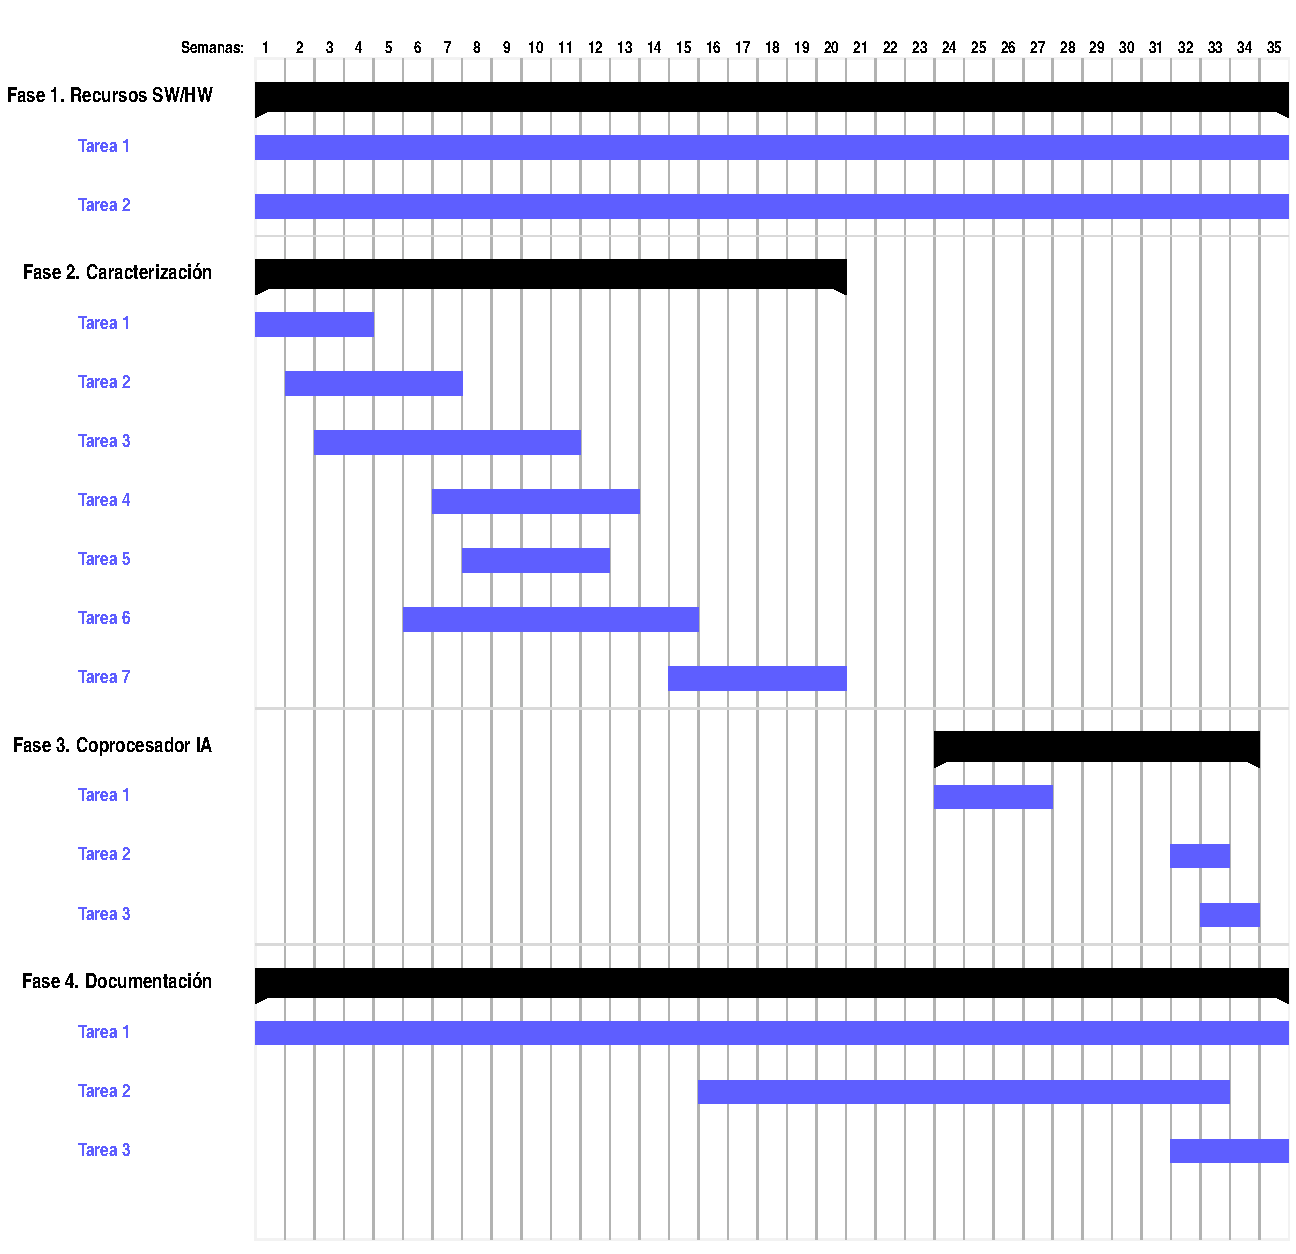
\includegraphics[width=14cm]{Figuras/Gantt.pdf}
    \caption{Diagrama de Gantt del desarrollo del trabajo.}
    \label{fig:gantt}
\end{figure}


%\section{Análisis de los resultados}
%
%Aqui irá un análisis de los resultados.

%capturas resultados en CI de github, analisis de los resultados de los distintos métodos.


